\documentclass[12pt,letter]{article}

%% \usepackage[fleqn]{amsmath}
\usepackage[margin=1in]{geometry}
\usepackage{amsmath,amsfonts,amsthm,bm}
\usepackage{breqn}
\usepackage{amsmath}
\usepackage{amssymb}
\usepackage{tikz}
\usepackage{algorithm2e}
\usepackage{siunitx}
\usepackage{graphicx}
\usepackage{subcaption}
%% \usepackage{datetime}
\usepackage{multirow}
\usepackage{multicol}
\usepackage{mathrsfs}
\usepackage{fancyhdr}
\usepackage{fancyvrb}
\usepackage{parskip} %turns off paragraph indent
\pagestyle{fancy}

\usetikzlibrary{arrows}

\DeclareMathOperator*{\argmin}{argmin}
\newcommand*{\argminl}{\argmin\limits}

\newcommand{\mathleft}{\@fleqntrue\@mathmargin0pt}
\newcommand{\R}{\mathbb{R}}
\newcommand{\Z}{\mathbb{Z}}
\newcommand{\N}{\mathbb{N}}
\newcommand{\indep}{\perp \!\!\! \perp}

\setcounter{MaxMatrixCols}{20}

\usepackage{listings}

\begin{document}

\rhead{(Bill)Yuan Liu, student \#: 996954078\\ Date: 2020/02/23}
\lhead{CSC2506 - Assignment 1}

Related code for the assignment can be found at A1.jmd

\section{Decision Theory}
\begin{align*}
\begin{tabular}{c|cc}
  Action & Spam & Not spam \\ \hline
  Show   & 10 & 0 \\
  Folder & 1  & 50 \\
  Delete & 0  & 200
\end{tabular}  
\end{align*}
\begin{enumerate}
\item Plot the expected wasted user time for each of the three possible actions, as a function of the probability of spam: $p(\textnormal{spam}|\textnormal{email})$
\begin{verbatim}
losses = [[10, 0],
          [1, 50],
          [0, 200]]
num_actions = length(losses)

function expected_loss_of_action(prob_spam, action)
    a = Array{Float64}(undef, size(prob_spam)[1],2)
    a[:,1] = prob_spam
    a[:,2] = 1.0 .- prob_spam
    b = losses[action]
    c = a * b
end

prob_range = range(0., stop=1., length=500)

text_actions = ["show", "foler", "delete"]

using Plots

for action in 1:num_actions
  display(plot!(prob_range, 
                expected_loss_of_action(prob_range, action),
                label=text_actions[action],
                title="Expected Loss of Actions",
                xlabel="p(spam)",
                ylabel="loss"))
end
savefig("1_1_expected_loss_of_action.png")
\end{verbatim}
  
  \pagebreak
  
\begin{figure}[h]
  \centering
  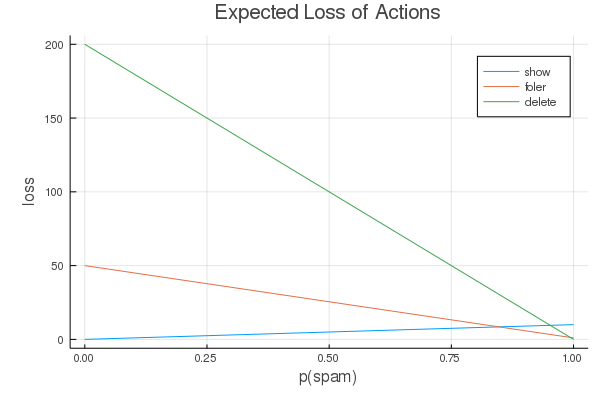
\includegraphics[width=14cm,keepaspectratio]{imgs/1_1_expected_loss_of_actions.png}
\end{figure}

\item Write a function that computes the optimal action given the probability of spam.
  
\begin{verbatim}
function optimal_action(prob_spam)
    out = zeros(size(prob_spam)[1], num_actions)
    for action in 1:num_actions
        out[:,action] = expected_loss_of_action(prob_range, action)
    end
    findmin(out, dims=2)
end
\end{verbatim}

  \pagebreak
  
\item Plot the expected loss of the optimal action as a function of the probability of spam.
  Color the line according to the optimal action for that probability of spam.

\begin{verbatim}
prob_range = range(0, stop=1., length=500)
best = optimal_action(prob_range)
optimal_losses = best[1]
optimal_actions = getindex.(best[2],2)
plot(prob_range, optimal_losses, linecolor=optimal_actions)
\end{verbatim}

\begin{figure}[h]
  \centering
  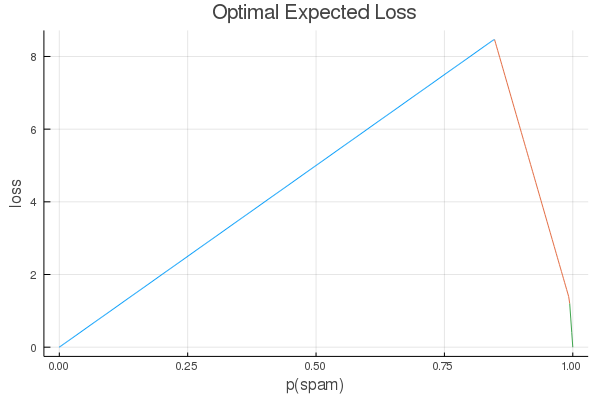
\includegraphics[width=14cm,keepaspectratio]{imgs/1_3.png}
\end{figure}
  
\item For exactly which range of the probabilities of an email being spam should we delete an email? Find the exact answer by hand using algebra.
  
  Solve for intersections of action pair (folder,delete):\\
  \begin{align*}
    p +50(1-p) &= 200(1-p)\\
    p + 50 -50p &= 200 - 200p\\
    151p &= 150\\
    p &= 150/151
  \end{align*}

  Deleting an email is optimal for $p(spam) \in [150/151,1]$.
\end{enumerate}

\pagebreak

\section{Regression}

\subsection{Manually Derived Linear Regression}
\begin{enumerate}
\item What happens if $n < m$?\\
  
  Then, the problem is underconstrained for $Y=X^T\beta + \epsilon$ and there exists multiple solutions.\\
  $Y=X^T(B+B'), \forall B' \in Nullspace(X^T)$\\
  $\beta^*=X(X^TX)^{-1}Y \implies X^T\beta^* = X^TX(X^TX)^{-1}Y = Y $\\
  $(\beta-\beta^*)^T\beta^* = (\beta-\beta^*)^TX(X^TX)^{-1}Y = (X^T\beta-X^T\beta^*)(X^TX)^{-1}Y = 0$\\
  Thus, $\beta^*=X(X^TX)^{-1}Y$ works.
  
\item What are the expectation and covariance matrix of $\hat{\beta}$, for a given true value of $\beta$?
  \begin{align*}
    E[\hat{\beta}] &= E[(XX^T)^{-1} XY]\\
                   &= E[(XX^T)^{-1} XX^T\beta+\epsilon], \epsilon \sim \mathcal{N}(0,\sigma^2 I)\\
                   &= \beta\\
    Var(\hat{\beta}) &= Var((XX^T)^{-1} XX^T\beta+\epsilon)\\
                   &= Var(\epsilon)\\
                   &= \sigma^2 I
  \end{align*}
\item Show that maximizing the likelihood is equivalent to minimizing the squared error $\sum_i(y_i - x_i \beta)^2$.
  \begin{align*}
    l(\theta|D) &= log\ p(\theta|D) = log \Pi_i \mathcal{N}(x_i^T\beta, \sigma^2)\\
    max l(\theta|D) &= min -l(\theta|D)\\
    -l(\theta|D) &= -\sum_i log \frac{1}{2 \pi \sigma^2} e^{-\frac{(y_i-x_i^T \beta)^2}{2\sigma^2}}\\
    \frac{\partial (-l(\theta|D))}{\partial \beta} &= 0 \\
                &= \frac{\partial \sum_i \frac{(y_i-x_i^T \beta)^2}{2\sigma^2}}{\partial \beta}\\
                &= \frac{2\sum_i (y_i-x_i^T \beta) (-x_i) }{2\sigma^2}
  \end{align*}
  Thus, minimizing likelihood is equivalent to minimzing $\sum_i (y_i-x_i^T \beta)^2$.\\

  \pagebreak
  
  \item Write the squared error in vector notation, (see above hint), expand the expression, and collect like terms.
    
\begin{align*}
  (y_i-x_i^T \beta)^2 &= (y_i-x_i^T \beta)^T(y_i-x_i^T \beta), y_i \in \R, x_i \in \R^m, \beta \in \R^m\\
                      &= (y_i-x_i^T \beta)^T(y_i-x_i^T \beta)\\
                      &= y_i^2 - y_i x_i^T \beta - \beta^T x_i y_i + \beta^T x_i  x_i^T \beta\\
                      &= y_i^2 - 2 y_i x_i^T \beta + (x_i^T \beta)^2\\
  \sum_i (y_i-x_i^T \beta)^2 &= y^T y - 2 y^T X^T \beta + (X^T \beta)^T (X^T \beta)\\
\end{align*}

  \item Use the likelihood expression to write the negative log-likelihood. Write the
derivative of the negative log-likelihood with respect to $\beta$, set equal to zero, and solve
to show the maximum likelihood estimate $\hat{\beta}$ as above.

\begin{align*}
  -l(\theta|D) &= -\sum_i log \frac{1}{2 \pi \sigma^2} e^{-\frac{(y_i-x_i^T \beta)^2}{2\sigma^2}}\\
  \frac{\partial (-l(\theta|D))}{\partial \beta} &= 0\\
               &= \frac{\partial \sum_i \frac{(y_i-x_i^T \beta)^2}{2\sigma^2}}{\partial \beta}\\
               &= \frac{\partial}{\partial \beta}(\frac{y^T y - 2 y^T X^T \beta + (X^T \beta)^T (X^T \beta)}{2\sigma^2})\\
               &= \frac{\partial}{\partial \beta}( - 2 y^T X^T \beta + (X^T \beta)^T (X^T \beta))\\
               &= - 2 (y^T X^T)^T + \frac{\partial (X^T\beta)^T}{\partial \beta}(X^T \beta) +  \frac{\partial (X^T \beta)^T }{\partial \beta} (X^T \beta)^T\\
               &= -2 X y + 2 X X^T \beta\\
  X X^T \beta &= Xy \\
  \beta &= (X X^T)^{-1} X y \\
\end{align*}

\end{enumerate}

\pagebreak

\subsection{Toy Data}

\begin{enumerate}
\item Write a function which produces a batch of data $x \sim \text{Uniform}(0,20)$ and $y = target\_f(x)$
\begin{verbatim}
function sample_batch(target_f, batch_size)
  x = 20.0 * rand(1, batch_size)
  y = target_f(x)
  return (x,y)
end
\end{verbatim}
  
  \begin{figure}[h]
    \centering
    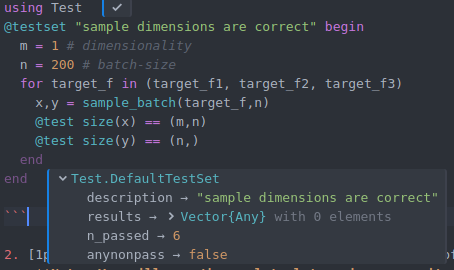
\includegraphics[width=13cm,keepaspectratio]{imgs/test1.png}
  \end{figure}
  
\item For all three targets, plot a $n=1000$ sample of the data.
\begin{verbatim}
using Plots

x1,y1 = sample_batch(target_f1,1000)
plot_f1 = plot(x1[1,:],y1,seriestype=:scatter,
     title="f1 samples",
     xlabel="x",
     ylabel="y",
     label="sample")

x2,y2 = sample_batch(target_f2,1000)
plot_f2 = plot(x2[1,:],y2,seriestype=:scatter,
     title="f2 samples",
     xlabel="x",
     ylabel="y",
     label="sample")

x3,y3 = sample_batch(target_f3,1000)
plot_f3 = plot(x3[1,:],y3,seriestype=:scatter,
     title="f3 samples",
     xlabel="x",
     ylabel="y",
     label="sample")
\end{verbatim}

  \begin{figure}[h]
    \centering
    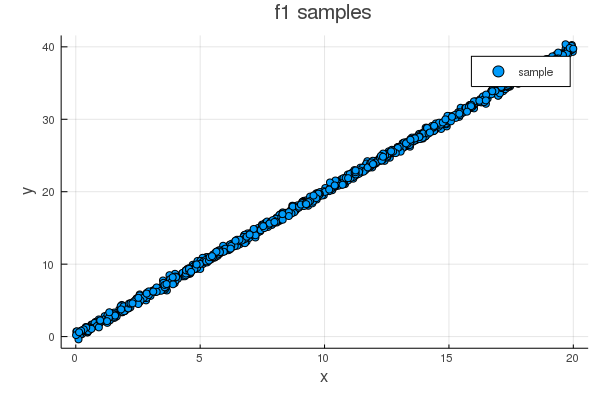
\includegraphics[width=12cm,keepaspectratio]{imgs/2_2_2_1.png}
  \end{figure}

  \begin{figure}[h]
    \centering
    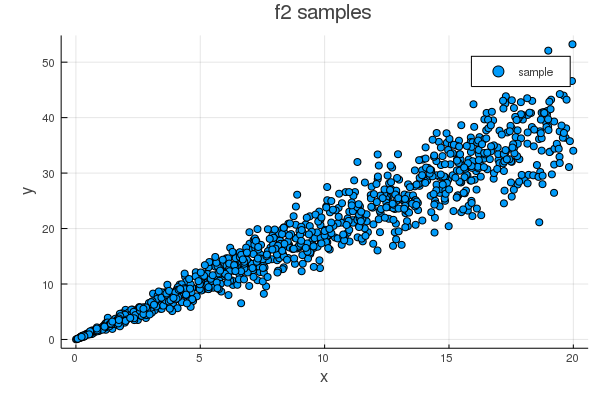
\includegraphics[width=12cm,keepaspectratio]{imgs/2_2_2_2.png}
  \end{figure}

    \begin{figure}[h]
    \centering
    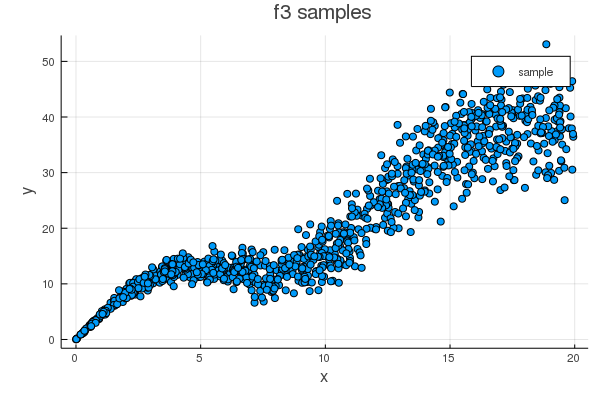
\includegraphics[width=12cm,keepaspectratio]{imgs/2_2_2_3.png}
  \end{figure}
  
\end{enumerate}

\subsection{Linear Regression Model with $\beta$ MLE}

\begin{enumerate}
\item Program the function that computes the the maximum likelihood estimate given $X$ and $Y$. Use it to compute the estimate $\hat \beta$ for a $n=1000$ sample from each target function.  
\begin{verbatim}
function beta_mle(X,Y)
  beta = inv(X*X') * X * Y
  return beta
end

n=1000 # batch_size

x_1, y_1 = sample_batch(target_f1,1000)
beta_mle_1 = beta_mle(x_1, y_1)

x_2, y_2 = sample_batch(target_f2,1000)
beta_mle_2 = beta_mle(x_2, y_2)

x_3, y_3 = sample_batch(target_f3,1000)
beta_mle_3 = beta_mle(x_3, y_3)
\end{verbatim}

\item For each function, plot the linear regression model given by $Y \sim \mathcal{N}(X^T \beta, \sigma^2I)$ for $\sigma=1$. This plot should have the line of best fit given by the maximum likelihood estimate, as well as a shaded region around the line corresponding to plus/minus one standard deviation (i.e. the fixed uncertainty $\sigma = 1.0$). Using Plots.jl this shaded uncertainty region can be achieved with the ribbon keyword argument. Display 3 plots, one for each target function, showing samples of data and maximum likelihood estimate linear regression model.

  Linear regression training with a constant bias, making $\beta=[\beta_1, \beta_2]$), was tested and makes very little difference since bias is very close to 0, so a scalar $\beta$ for estimating slope suffices.
  \pagebreak
\begin{lstlisting}[
    mathescape,
    columns=fullflexible,
    basicstyle=\ttfamily\footnotesize,breaklines=true
    ]
using Distributions

x=0:20

fit_1 = x ->  $\beta$_mle_1[1] * x
plot(plot_f1)
plot!(fit_1, 0,20, 
      title="f1 Samples and Linear Fit",
      ribbon=1.0,
      label="fit")
savefig("imgs/2_3_2_1.png")

fit_2 = x ->  $\beta$_mle_2[1] * x
plot(plot_f2)
plot!(fit_2, 0,20,
      title="f2 Samples and Linear Fit",
      ribbon=1.0,
      label="fit")
savefig("imgs/2_3_2_2.png")

fit_3 = x ->  $\beta$_mle_3[1] * x
plot_f3
plot!(fit_3, 0,20,
      title="f3 Samples and Linear Fit",
      ribbon=1.0,
      label="fit")
savefig("imgs/2_3_2_3.png")
\end{lstlisting}
  
\begin{figure}[h]
  \centering
    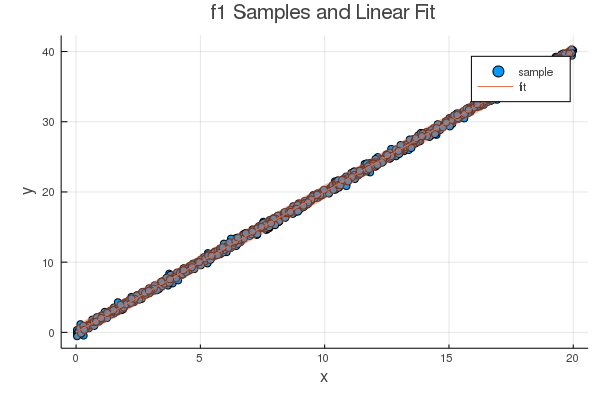
\includegraphics[width=13cm,keepaspectratio]{imgs/2_3_2_1.png}
  \end{figure}
\pagebreak
\begin{figure}[h]
  \centering
  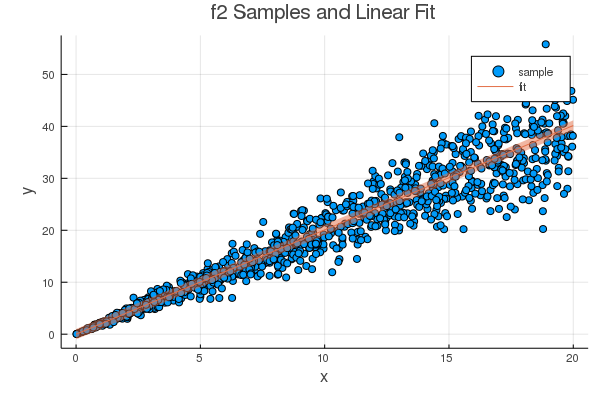
\includegraphics[width=13cm,keepaspectratio]{imgs/2_3_2_2.png}
  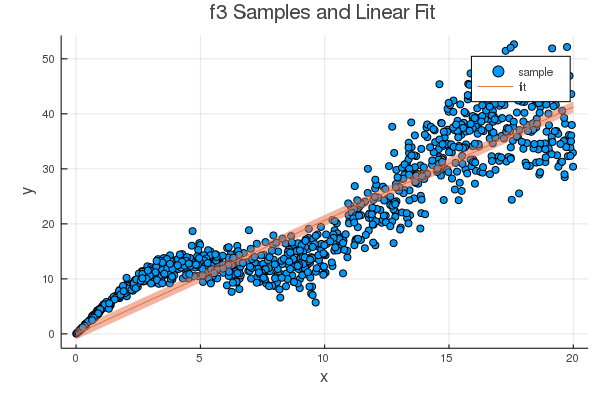
\includegraphics[width=13cm,keepaspectratio]{imgs/2_3_2_3.png}
\end{figure}

\end{enumerate}

\pagebreak

\subsection{Log-likelihood of Data Under Model}
\begin{enumerate}
\item Write code for the function that computes the likelihood of $x$ under the Gaussian distribution $\mathcal{N}(\mu,\sigma)$. For reasons that will be clear later, this function should be able to broadcast to the case where $x, \mu, \sigma$ are all vector valued and return a vector of likelihoods with equivalent length, i.e., $x_i \sim \mathcal{N}(\mu_i,\sigma_i)$.
\begin{lstlisting}[
    mathescape,
    columns=fullflexible,
    basicstyle=\ttfamily\footnotesize,breaklines=true
    ]
function gaussian_log_likelihood($\mu$, $\sigma$, x)
  log.(1. ./ sqrt.(2*pi.*$\sigma$.^2)) .+ (-0.5 .* ((x.-$\mu$).^2)/$\sigma$.^2)
end
\end{lstlisting}

Test Gaussian likelihood against standard implementation.
\begin{figure}[h]
  \centering
  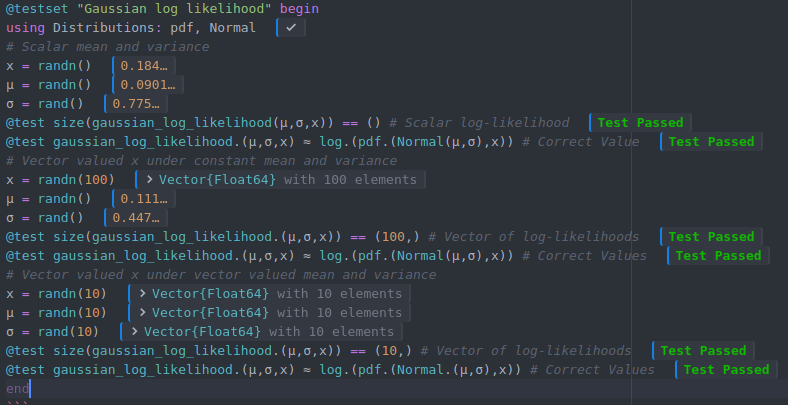
\includegraphics[width=16cm, keepaspectratio]{imgs/test2.png}
\end{figure}

\item Use your gaussian log-likelihood function to write the code which computes the negative log-likelihood of the target value $Y$ under the model $Y \sim \mathcal{N}(X^T\beta, \sigma^2*I)$ for a given value of $\beta$.
  
\begin{lstlisting}[
    mathescape,
    columns=fullflexible,
    basicstyle=\ttfamily\footnotesize,breaklines=true
    ]
function lr_model_nll($\beta$,x,y;$\sigma$=1.)
  mu = (x' * $\beta$)
  sum(-1 .* gaussian_log_likelihood.(mu, $\sigma$, y))
end
\end{lstlisting}

\pagebreak

\item Use this function to compute and report the negative-log-likelihood of a $n\in \{10,100,1000\}$ batch of data under the model with the maximum-likelihood estimate $\hat\beta$ and $\sigma \in \{0.1,0.3,1.,2.\}$ for each target function.
  
\begin{lstlisting}[
    mathescape,
    columns=fullflexible,
    basicstyle=\ttfamily\footnotesize,breaklines=true
    ]
for n in (10,100,1000)
    println("--------  $\$$n  ------------")
    for target_f in (target_f1,target_f2, target_f3)
      println("--------  $\$$target_f  ------------")
      for $\sigma$_model in (0.1,0.3,1.,2.)
        println("--------  $\$\sigma$_model  ------------")
        x,y = sample_batch(target_f,n)
        $\beta$_mle = beta_mle(x,y)
        nll = lr_model_nll($\beta$_mle,x,y,$\sigma$=$\sigma$_model)
        println("Negative Log-Likelihood: $\$$nll")
      end
    end
end
\end{lstlisting}

\item For each target function, what is the best choice of $\sigma$?\\
  Using N=10:\\
  \begin{tabular}{|c|c|c|c|c|}
    \hline
    & $\sigma=0.1$ & $\sigma=0.3$ & $\sigma=1.0$ & $\sigma=2.0$ \\\hline
    target\_f1 & 29.33 & 4.91 & 9.49 & 16.24 \\\hline
    target\_f2 & 3855.20 & 679.16 & 53.88 & 31.19 \\\hline
    target\_f3 & 18084.52 & 805.28 & 136.68 & 31.27 \\\hline
  \end{tabular}\\
  \\
  We observed best choice of $\sigma_{target\_f1} = 0.3$, $\sigma_{target\_f2} = 2.0$, $\sigma_{target\_f1} = 2.0$.
  
  Using N=100:\\
  \begin{tabular}{|c|c|c|c|c|}
    \hline
    & $\sigma=0.1$ & $\sigma=0.3$ & $\sigma=1.0$ & $\sigma=2.0$ \\\hline
    target\_f1 & 290.15 & 29.81 & 96.2 & 162.2 \\\hline
    target\_f2 & 53752.83 & 6605.53 & 489.89 & 281.52 \\\hline
    target\_f3 & 123286.74 & 14524.38 & 1109.84 & 413.30 \\\hline
  \end{tabular}\\
  \\
  We observed best choice of $\sigma_{target\_f1} = 0.3$, $\sigma_{target\_f2} = 2.0$, $\sigma_{target\_f1} = 2.0$.
  
  Using N=1000:\\
  \begin{tabular}{|c|c|c|c|c|}
    \hline
    & $\sigma=0.1$ & $\sigma=0.3$ & $\sigma=1.0$ & $\sigma=2.0$ \\\hline
    target\_f1 & 2840.99 & 205.14 & 965.24 & 1623.16 \\\hline
    target\_f2 & 588157.09 & 64999.86 & 7775.36 & 3134.97 \\\hline
    target\_f3 & 1286740.39 & 128972.94 & 12401.60 & 4612.70 \\\hline
  \end{tabular}\\
  \\
  We observed best choice of $\sigma_{target\_f1} = 0.3$, $\sigma_{target\_f2} = 2.0$, $\sigma_{target\_f1} = 2.0$.

\end{enumerate}
\pagebreak
\subsection{Automatic Differentiation with Maximizing Likelihood}

For a random value of $\beta$, $\sigma$, and n = 100 sample from a target function, use automatic differentiation to compute the derivative of the negative log-likelihood of the sampled data with respect β. Test that this is equivalent to the hand-derived value.\\

\begin{lstlisting}[
    mathescape,
    columns=fullflexible,
    basicstyle=\ttfamily\footnotesize,breaklines=true
    ]
using Zygote: gradient

@testset "Gradients wrt parameter" begin
$\beta$_test = randn()
$\sigma$_test = rand()
x,y = sample_batch(target_f1,100)
ad_grad = gradient( (bb, xx,yy, sigma) -> lr_model_nll(bb,xx,yy,$\sigma$=sigma), $\beta$_test, x, y, $\sigma$_test)
hand_derivative = ((-2 * x * y .+ 2* x * x' * $\beta$_test)./(2*$\sigma$_test^2))[1]
@test ad_grad[1] $\approx$ hand_derivative
end
\end{lstlisting}

\begin{figure}[h]
  \centering
  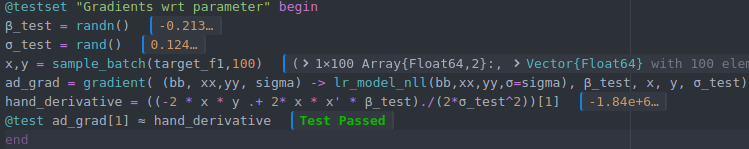
\includegraphics[width=17cm,keepaspectratio]{imgs/test3.png}
\end{figure}

\pagebreak

\subsubsection{Train Linear Regression Model with Gradient Descent}

\begin{enumerate}
\item Write a function train\_lin\_reg that accepts a target function and an initial
estimate for $\beta$ and some hyperparameters for batch-size, model variance, learning rate,
and number of iterations.
\begin{lstlisting}[
    mathescape,
    columns=fullflexible,
    basicstyle=\ttfamily\footnotesize,breaklines=true
    ]
function train_lin_reg(target_f, β_init; bs= 100, lr = 1e-6, iters=1000, $\sigma$_model = 1. )
    $\beta$_curr = $\beta$_init
    for i in 1:iters
      x,y = sample_batch(target_f,bs)
      grad_$\beta$ = gradient((bb, xx,yy, sigma) -> lr_model_nll(bb,xx,yy,$\sigma$=sigma), $\beta$_curr, x, y, $\sigma$_model)[1]
      $\beta$_curr = $\beta$_curr - grad_$\beta$ * lr
    end
    $\beta$_curr
end
\end{lstlisting}

\item For each target function, start with an initial parameter $\beta$, learn an estimate for $\beta$_learned by gradient descent. Then plot a $n=1000$ sample of the data and the learned linear regression model with shaded region for uncertainty corresponding to plus/minus one standard deviation.
\begin{lstlisting}[
    mathescape,
    columns=fullflexible,
    basicstyle=\ttfamily\footnotesize,breaklines=true
    ]
$\beta$_init = [randn(), randn(), randn()] # Initial parameter
targets = [target_f1, target_f2, target_f3]
$\beta$_learned = train_lin_reg.(targets, $\beta$_init; bs= 100, lr = 1e-6, iters=1000, $\sigma$_model = 1. )
x=0:20
plot(plot_f1)
plot!(x->$\beta$_learned[1]*x, x,
      title="f1 Samples and Linear Fit",
      xlabel="x",
      ylabel="y",
      ribbon=1.0,
      label="fit")
savefig("imgs/2_5_1_2_1.png")
plot(plot_f2)
plot!(x->$\beta$_learned[2]*x, x,
      title="f2 Samples and Linear Fit",
      xlabel="x",
      ylabel="y",
      ribbon=1.0,
      label="fit")
savefig("imgs/2_5_1_2_2.png")
plot(plot_f3)
plot!(x->$\beta$_learned[3]*x, x,
      title="f3 Samples and Linear Fit",
      xlabel="x",
      ylabel="y",
      ribbon=1.0,
      label="fit")
savefig("imgs/2_5_1_2_3.png")      
\end{lstlisting}
\pagebreak
\begin{figure}[h]
  \centering
  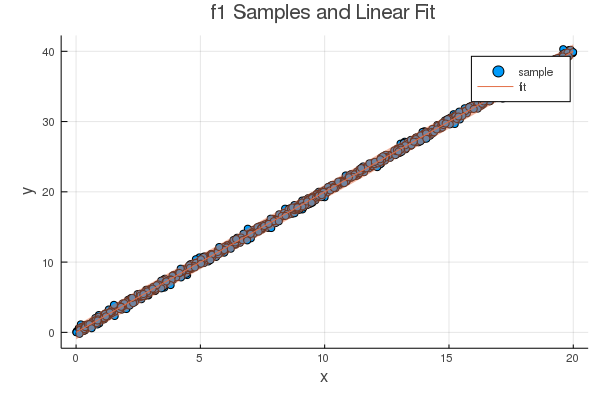
\includegraphics[width=12.5cm,keepaspectratio]{imgs/2_5_1_2_1.png}
\end{figure}
\begin{figure}[h]
  \centering
  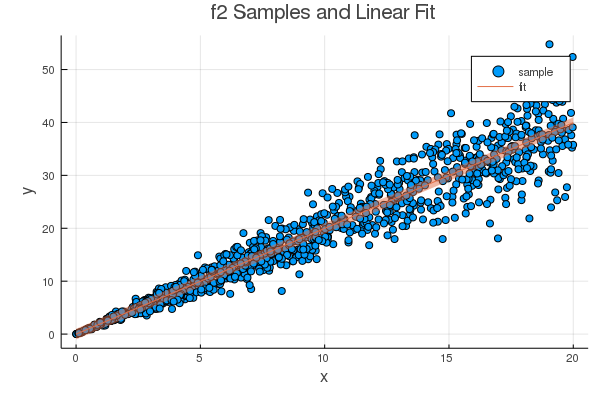
\includegraphics[width=12.5cm,keepaspectratio]{imgs/2_5_1_2_2.png}
\end{figure}
\begin{figure}[h]
  \centering
  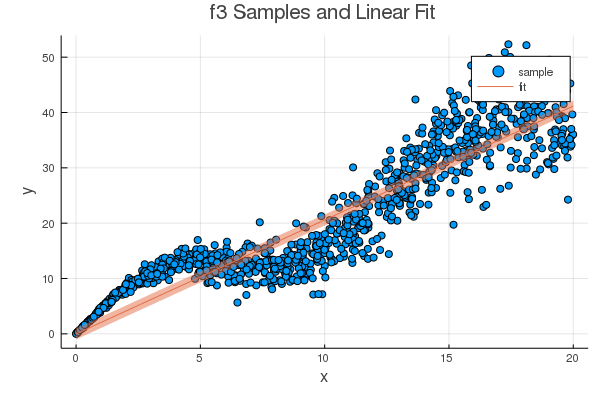
\includegraphics[width=12cm,keepaspectratio]{imgs/2_5_1_2_3.png}
\end{figure}
\end{enumerate}
\pagebreak
\subsubsection{Non-linear Regression with a Neural Network}
\begin{enumerate}
\item Write the code for a fully-connected neural network (multi-layer perceptron) with one 10-dimensional hidden layer and a tanh nonlinearirty. You must write this yourself using only basic operations like matrix multiply and tanh, you may not use layers provided by a library. This network will output the mean vector, test that it outputs the correct shape for some random parameters.
\begin{lstlisting}[
    mathescape,
    columns=fullflexible,
    basicstyle=\ttfamily\footnotesize,breaklines=true
    ]
# Neural Network Function
function neural_net(x,$\theta$)
  hidden = 0.5 .* tanh.($\theta$[1] * x .+ $\theta$[2]) .+ 0.5
  out = $\theta$[3] * (hidden .+ $\theta$[4])
  out[:]
end
\end{lstlisting}
% n = 100
% h = 10
% $\theta$ = [randn((h,1)), randn((h,1)), randn(1,h), randn(h,1)]
% @testset "neural net mean vector output" begin
% x,y = sample_batch(target_f1,n)
% $\mu$ = neural_net(x,$\theta$)
% @test size($\mu$) == (n,)
% end
\begin{figure}[h]
  \centering
  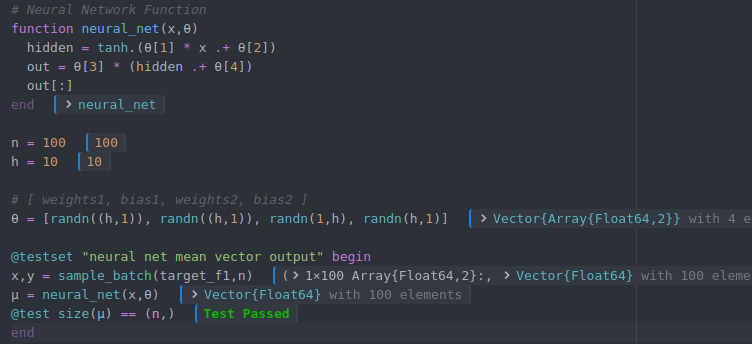
\includegraphics[width=15cm,keepaspectratio]{imgs/test4.png}
\end{figure}

\pagebreak

\item Write the code that computes the negative log-likelihood for this model where the mean is given by the output of the neural network and $\sigma = 1.0$

\begin{lstlisting}[
    mathescape,
    columns=fullflexible,
    basicstyle=\ttfamily\footnotesize,breaklines=true
    ]
function nn_model_nll($\theta$,x,y;$\sigma$=1)
  mu = neural_net(x,$\theta$)
  sum(-1 .* gaussian_log_likelihood.(mu, $\sigma$, y))
end
\end{lstlisting}

\item Write a function, train\_nn\_reg, that accepts a target function and an initial estimate for $\theta$ and some hyperparameters for batch-size, model variance, learning rate, and number of iterations.

\begin{lstlisting}[
    mathescape,
    columns=fullflexible,
    basicstyle=\ttfamily\footnotesize,breaklines=true
    ]
function train_nn_reg(target_f, $\theta$_init; bs= 200, lr = 1e-5, iters=1000, $\sigma$_model = 1. )
    # momentum
    b = 0.99
    v = $\theta$_init .* 0
    $\theta$_curr = $\theta$_init
    for i in 1:iters
      x,y = sample_batch(target_f,bs)
      grad_$\theta$ = gradient(
        (theta, xx, yy, sigma) -> nn_model_nll(theta,xx,yy,$\sigma$=sigma),
        $\theta$_curr, x, y, $\sigma$_model)[1]
      v = b .* v + (1.0 - b) .* grad_$\theta$
      $\theta$_curr = $\theta$_curr - lr .* v
    end
    $\theta$_curr
end
\end{lstlisting}

\item For each target function, start with an initialization of the network parameters, $\theta$, use your train function to minimize the negative log-likelihood and find an estimate for $\theta$_learned by gradient descent. Then plot a $n=1000$ sample of the data and the learned regression model with shaded uncertainty bounds given by $\sigma = 1.0$

\begin{lstlisting}[
    mathescape,
    columns=fullflexible,
    basicstyle=\ttfamily\footnotesize,breaklines=true
    ]
h=10
$\theta$_init = [  0.001*[randn((h,1)), randn((h,1)), randn(1,h), randn(h,1)],
            0.001*[randn((h,1)), randn((h,1)), randn(1,h), randn(h,1)],
            0.001*[randn((h,1)), randn((h,1)), randn(1,h), randn(h,1)],
         ]

targets = [target_f1, target_f2, target_f3]

$\theta$_learned = train_nn_reg.(targets, $\theta$_init; bs= 300, lr = 1e-5, iters=4000, $\sigma$_model = 1.0 )

# plot data samples and learned regression

x = reshape([i for i =0:1:20],1, :)

mu = neural_net(x,$\theta$_learned[1])
p1 = plot(x1[1,:],y1,seriestype=:scatter,
     title="f1 Samples and Non-Linear Mean Fit, sigma=1",
     xlabel="x",
     ylabel="y",
     label="sample")
plot!(x[:],mu[:],
      linewidth = 2,
      linecolor = :cyan,
      ribbon=1.0,
      label="fit")
savefig("imgs/2_5_2_4_1.png")
      
mu = neural_net(x,$\theta$_learned[2])
plot(x2[1,:],y2,seriestype=:scatter,
          title="f2 Samples and Non-Linear Mean Fit, sigma=1",
          xlabel="x",
          ylabel="y",
          label="sample")
plot!(x[:],mu[:],
      linewidth = 2,
      linecolor = :cyan,
      ribbon=1.0,
      label="fit")
savefig("imgs/2_5_2_4_2.png")

mu = neural_net(x,$\theta$_learned[3])
plot(x3[1,:],y3,seriestype=:scatter,
          title="f3 Samples and Non-Linear Mean Fit, sigma=1",
          xlabel="x",
          ylabel="y",
          label="sample")
plot!(x[:],mu[:],
      linewidth = 2,
      linecolor = :cyan,
      ribbon=1.0,
      label="fit")
savefig("imgs/2_5_2_4_3.png")
\end{lstlisting}

\pagebreak

\begin{figure}[h]
  \centering
  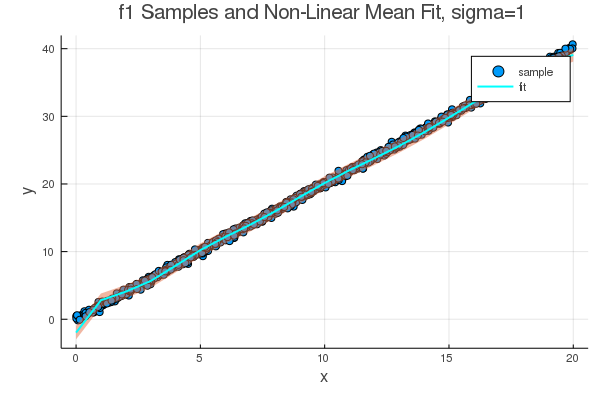
\includegraphics[width=13cm,keepaspectratio]{imgs/2_5_2_4_1.png}
  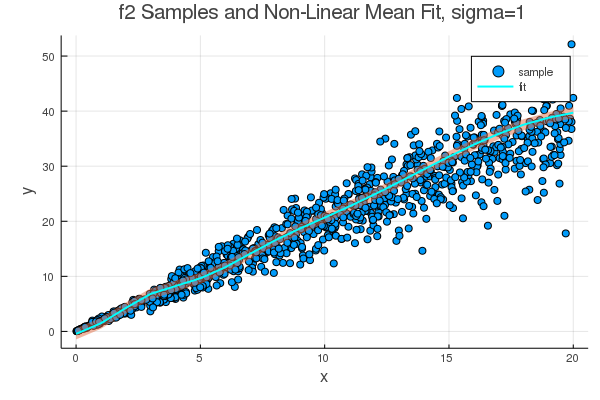
\includegraphics[width=13cm,keepaspectratio]{imgs/2_5_2_4_2.png}
\end{figure}
% \begin{figure}[h]
%   \centering
%   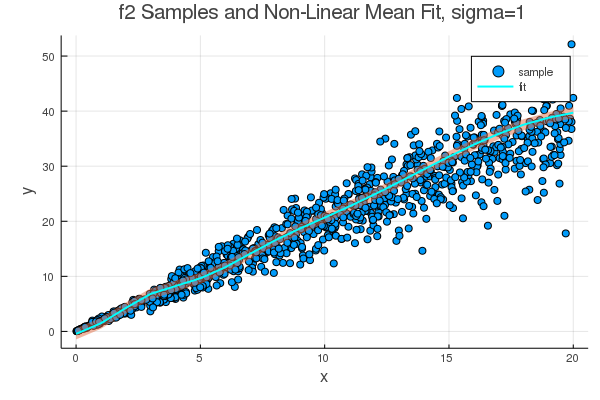
\includegraphics[width=13cm,keepaspectratio]{imgs/2_5_2_4_2.png}
% \end{figure}
\begin{figure}[h]
  \centering
  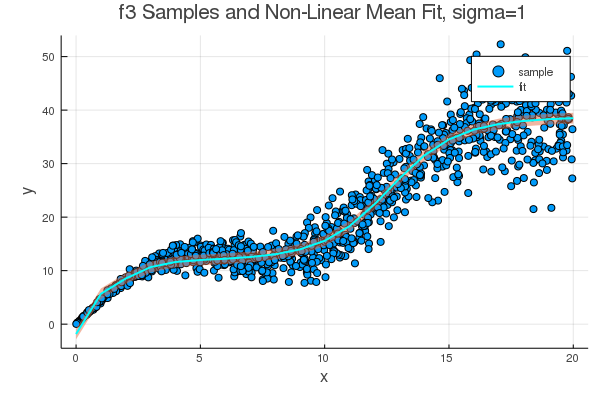
\includegraphics[width=13cm,keepaspectratio]{imgs/2_5_2_4_3.png}
\end{figure}
\end{enumerate}

\pagebreak

\subsubsection{Non-linear Regression and Input-dependent Variance with a Neural Network}

\begin{enumerate}
  
\item Write the code for a fully-connected neural network (multi-layer perceptron) with one 10-dimensional hidden layer and a `tanh` nonlinearirty, and outputs both a vector for mean and $\log \sigma$. Test the output shape is as expected.

\pagebreak
  
\begin{lstlisting}[
    mathescape,
    columns=fullflexible,
    basicstyle=\ttfamily\footnotesize,breaklines=true
    ]
function neural_net_w_var(x, $\theta$, stat_count, stat_mean, stat_var; training=true)

  hidden_theta_1 = $\theta$[1][1] * x .+ $\theta$[1][2]

  new_count = stat_count + size(x)[2]

  #batch normalization for nodes responsible for mean estimation
  if training == true
    avg1 = sum(hidden_theta_1, dims=2) ./ size(x)[2]
    var1 = sum((hidden_theta_1 .- avg1).^2, dims=2) ./ size(x)[2]
    hidden_theta_1_normalized = (hidden_theta_1 .- avg1) ./ sqrt.(var1 .+ 1e-10)
    hidden_theta_1_activation = $\theta$[1][9] * ($\theta$[1][5] .* (tanh.(hidden_theta_1_normalized .-1.1)) .+ $\theta$[1][6])

    # println(size(stat_mean[1][1]))
    stat_mean_new_1 = stat_mean[1][1] .* 0.98 .+ avg1 .* 0.02
    stat_var_new_1 = stat_var[1][1] .* 0.98 .+ var1 .* 0.02

    avg12 = sum(hidden_theta_1_activation, dims=2) ./ size(hidden_theta_1_activation)[2]
    var12 = sum((hidden_theta_1_activation .- avg12).^2, dims=2) ./ size(hidden_theta_1_activation)[2]
    hidden_theta_2_normalized = (hidden_theta_1_activation .- avg12) ./ sqrt.(var12 .+ 1e-10)
    hidden_theta_2_activation = $\theta$[1][7] .* (tanh.(hidden_theta_2_normalized .-1.1)) .+ $\theta$[1][8]

    stat_mean_new_12 = stat_mean[1][2] .* 0.98 .+ avg12 .* 0.02
    stat_var_new_12 = stat_var[1][2] .* 0.98 .+ var12 .* 0.02

  else
    hidden_theta_1_normalized = (hidden_theta_1 .- stat_mean[1][1]) ./ sqrt.(stat_var[1][1] .+ 1e-10)
    hidden_theta_1_activation = $\theta$[1][9] * ($\theta$[1][5] .* (tanh.(hidden_theta_1_normalized .-1.1)) .+ $\theta$[1][6])

    hidden_theta_2_normalized = (hidden_theta_1_activation .- stat_mean[1][2]) ./ sqrt.(stat_var[1][2] .+ 1e-10)
    hidden_theta_2_activation = $\theta$[1][7] .* (tanh.(hidden_theta_2_normalized .-1.1)) .+ $\theta$[1][8]

    stat_mean_new_1 = stat_mean[1][1]
    stat_var_new_1 = stat_var[1][1]

    stat_mean_new_12 = stat_mean[1][2]
    stat_var_new_12 = stat_var[1][2]
  end

  out_theta = $\theta$[1][4] * (hidden_theta_2_activation .+ $\theta$[1][3])

  hidden_log_variance_1 = $\theta$[2][1] * x .+ $\theta$[2][2]


  
  #batch normalization for nodes responsible for log variance estimation
  if training == true
    avg2 = sum(hidden_log_variance_1, dims=2) ./ size(x)[2]
    var2 = sum((hidden_log_variance_1 .- avg2).^2, dims=2) ./size(x)[2]
    hidden_log_variance_1_normalized = (hidden_log_variance_1 .- avg2) ./ sqrt.(var2 .+ 1e-10)
    hidden_log_variance_1_activation = $\theta$[2][9] * ($\theta$[2][5] .* (tanh.(hidden_log_variance_1_normalized .-1.1)) .+ $\theta$[2][6])

    stat_mean_new_2 = stat_mean[2][1] .* 0.98 .+ avg2 .* 0.02
    stat_var_new_2 = stat_var[2][1] .* 0.98 .+ var2 .* 0.02

    avg22 = sum(hidden_log_variance_1_activation, dims=2) ./ size(hidden_log_variance_1_activation)[2]
    var22 = sum((hidden_log_variance_1_activation .- avg2).^2, dims=2) ./size(hidden_log_variance_1_activation)[2]
    hidden_log_variance_2_normalized = (hidden_log_variance_1_activation .- avg22) ./ sqrt.(var22 .+ 1e-10)
    hidden_log_variance_2_activation = $\theta$[2][7] .* (tanh.(hidden_log_variance_2_normalized .-1.1)) .+ $\theta$[2][8]

    stat_mean_new_22 = stat_mean[2][2] .* 0.98 .+ avg22 .* 0.02
    stat_var_new_22 = stat_var[2][2] .* 0.98 .+ var22 .* 0.02

  else
    hidden_log_variance_1_normalized = (hidden_log_variance_1 .- stat_mean[2][1]) ./ sqrt.(stat_var[2][2] .+ 1e-10)
    hidden_log_variance_1_activation = $\theta$[2][9] * ($\theta$[2][5] .* (tanh.(hidden_log_variance_1_normalized .-1.1)) .+ $\theta$[2][6])

    hidden_log_variance_2_normalized = (hidden_log_variance_1_activation .- stat_mean[2][2]) ./ sqrt.(stat_var[2][2] .+ 1e-10)
    hidden_log_variance_2_activation = $\theta$[2][7] .* (tanh.(hidden_log_variance_2_normalized .-1.1)) .+ $\theta$[2][8]

    stat_mean_new_2 = stat_mean[2][1]
    stat_var_new_2 = stat_var[2][1]

    stat_mean_new_22 = stat_mean[2][2]
    stat_var_new_22 = stat_var[2][2]
  end

  out_log_variance = $\theta$[2][4] * (hidden_log_variance_2_activation .+ $\theta$[2][3])

  return (out_theta[:],
          out_log_variance[:],
          new_count,
          [[stat_mean_new_1, stat_mean_new_12],[stat_mean_new_2, stat_mean_new_22]],
          [[stat_var_new_1, stat_var_new_12], [stat_var_new_2, stat_var_new_22]])
end

$\theta$ = [[randn((h,1)), randn((h,1)), randn(h,1), randn(1,h), randn(h,1), randn(h,1), randn(h,1), randn(h,1), randn(h,h)],
     [randn((h,1)), randn((h,1)), randn(h,1), randn(1,h), randn(h,1), randn(h,1), randn(h,1), randn(h,1), randn(h,h)]]

h = 10

@testset "neural net mean and logsigma vector output" begin
n = 10
x,y = sample_batch(target_f1,n)
stat_count = $\theta$
stat_mean = [ [zeros((h,1)), zeros((h,1))], [zeros((h,1)), zeros((h,1))] ]
stat_var = [ [zeros((h,1)), zeros((h,1))], [zeros((h,1)), zeros((h,1))] ]
μ, logσ, _ = neural_net_w_var(x,$\theta$, stat_count, stat_mean, stat_var)
@test size(μ) == (n,)
@test size(logσ) == (n,)
end
\end{lstlisting}
\begin{figure}[h]
  \centering
  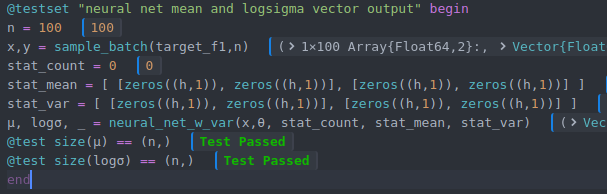
\includegraphics[width=15cm,keepaspectratio]{imgs/test5.png}
\end{figure}

\item Write the code that computes the negative log-likelihood for this model where the mean and $\log \sigma$ is given by the output of the neural network.

\begin{lstlisting}[
    mathescape,
    columns=fullflexible,
    basicstyle=\ttfamily\footnotesize,breaklines=true
    ]
function nn_with_var_model_nll($\theta$,x,y, stat_count, stat_mean, stat_var; training=true)
  mu, log_variance, new_count, new_mean, new_var = neural_net_w_var(x,$\theta$, stat_count, stat_mean, stat_var; training=true)
  sum(-1 .* gaussian_log_likelihood.(mu, sqrt.(exp.(log_variance)), y)), new_count, new_mean, new_var
end
\end{lstlisting}

\pagebreak

\item Write a function `train\_nn\_w\_var\_reg` that accepts a target function and an initial estimate for $\theta$ and some hyperparameters for batch-size, learning rate, and number of iterations.

\begin{lstlisting}[
    mathescape,
    columns=fullflexible,
    basicstyle=\ttfamily\footnotesize,breaklines=true
    ]
function train_nn_w_var_reg(target_f, $\theta$_init, stat_count, stat_mean, stat_var; bs= 100, lr = 1e-5, iters=10000)
  # update method: SGD with momentum
  b = 0.97
  v = $\theta$_init .* 0
  $\theta$_curr = $\theta$_init

  final_loss = Inf64

  for i in 1:iters
    x,y = sample_batch(target_f,bs)

    function ff(theta, xx, yy, s_count, s_mean, s_var)
      loss, s_count, s_mean, s_var = nn_with_var_model_nll(theta,xx,yy, s_count, s_mean, s_var; training=true)
      stat_count = s_count
      stat_mean = s_mean
      stat_var = s_var

      final_loss = loss

      if i % 100 == 0
          println("iter: ", i,", loss: ", loss)
      end

      loss
    end

    grad_$\theta$ = gradient(ff, $\theta$_curr, x, y, stat_count, stat_mean, stat_var)[1]

    v = b .* v + (1.0 - b) .* grad_$\theta$
    $\theta$_curr = $\theta$_curr - lr .* v

  end
  ($\theta$_curr, stat_count, stat_mean, stat_var, final_loss)
end
\end{lstlisting}

\pagebreak

\item For each target function, start with an initialization of the network parameters, $\theta$, learn an estimate for $\theta$\_learned by gradient descent. Then plot a $n=1000$ sample of the dataset and the learned regression model with shaded uncertainty bounds corresponding to plus/minus one standard deviation given by the variance of the predictive distribution at each input location (output by the neural network).

\begin{lstlisting}[
  mathescape,
  columns=fullflexible,
  basicstyle=\ttfamily\footnotesize,breaklines=true
  ]

h=10

$\theta$_init =  0.001 *  [ [[randn((h,1)), randn((h,1)), randn(h,1), randn(1,h), randn(h,1), randn(h,1), randn(h,1), randn(h,1), randn(h,h)],
                      [randn((h,1)), randn((h,1)), randn(h,1), randn(1,h), randn(h,1), randn(h,1), randn(h,1), randn(h,1), randn(h,h)]],
                     [[randn((h,1)), randn((h,1)), randn(h,1), randn(1,h), randn(h,1), randn(h,1), randn(h,1), randn(h,1), randn(h,h)],
                      [randn((h,1)), randn((h,1)), randn(h,1), randn(1,h), randn(h,1), randn(h,1), randn(h,1), randn(h,1), randn(h,h)]],
                     [[randn((h,1)), randn((h,1)), randn(h,1), randn(1,h), randn(h,1), randn(h,1), randn(h,1), randn(h,1), randn(h,h)],
                      [randn((h,1)), randn((h,1)), randn(h,1), randn(1,h), randn(h,1), randn(h,1), randn(h,1), randn(h,1), randn(h,h)]] ]

targets = [target_f1, target_f2, target_f3]

global stat_mean = [ [[zeros((h,1)), zeros((h,1))], [zeros((h,1)), zeros((h,1))]],
                     [[zeros((h,1)), zeros((h,1))], [zeros((h,1)), zeros((h,1))]],
                     [[zeros((h,1)), zeros((h,1))], [zeros((h,1)), zeros((h,1))]], ]

global stat_var =  [ [[zeros((h,1)), zeros((h,1))], [zeros((h,1)), zeros((h,1))]],
                     [[zeros((h,1)), zeros((h,1))], [zeros((h,1)), zeros((h,1))]],
                     [[zeros((h,1)), zeros((h,1))], [zeros((h,1)), zeros((h,1))]], ]

stat_count = [0, 0, 0]

ret = train_nn_w_var_reg.(targets, $\theta$_init, stat_count, stat_mean, stat_var; bs= 2000, lr = 4e-5, iters=10000)

global $\theta$_learned = map(x->x[1], ret)
global scount = map(x->x[2],ret)
global smean = map(x->x[3],ret)
global svar = map(x->x[4],ret)

# plot data samples and learned regression

support = reshape([i for i =0:0.01:20],1, :)

mu_1, log_variance_1 = neural_net_w_var(support,$\theta$_learned[1], scount[1], smean[1], svar[1]; training=false)

plot(x1[1,:],y1,seriestype=:scatter,
          title="f1 Samples and Non-Linear Fit",
          xlabel="x",
          ylabel="y",
          label="sample")
plot!(support[:],mu_1[:],
      linewidth = 2,
      linecolor = :cyan,
      ribbon=sqrt.(exp.(log_variance_1)),
      label="fit")

savefig("imgs/2_5_3_4_1.png")

mu_2, log_variance_2 = neural_net_w_var(support,$\theta$_learned[2], scount[2], smean[2], svar[2]; training=false)

plot(x2[1,:],y2,seriestype=:scatter,
          title="f2 Samples and Non-Linear Fit",
          xlabel="x",
          ylabel="y",
          label="sample")
plot!(support[:],mu_2[:],
      linewidth = 2,
      linecolor = :cyan,
      ribbon=sqrt.(exp.(log_variance_2)),
      label="fit")

savefig("imgs/2_5_3_4_2.png")

mu_3, log_variance_3 = neural_net_w_var(support,$\theta$_learned[3], scount[3], smean[3], svar[3]; training=false)

plot(x3[1,:],y3,seriestype=:scatter,
          title="f3 Samples and Non-Linear Fit",
          xlabel="x",
          ylabel="y",
          label="sample")
plot!(support[:],mu_3[:],
      linewidth = 2,
      linecolor = :cyan,
      ribbon=sqrt.(exp.(log_variance_3)),
      label="fit")

savefig("imgs/2_5_3_4_3.png")
\end{lstlisting}

\begin{figure}[h]
  \centering
  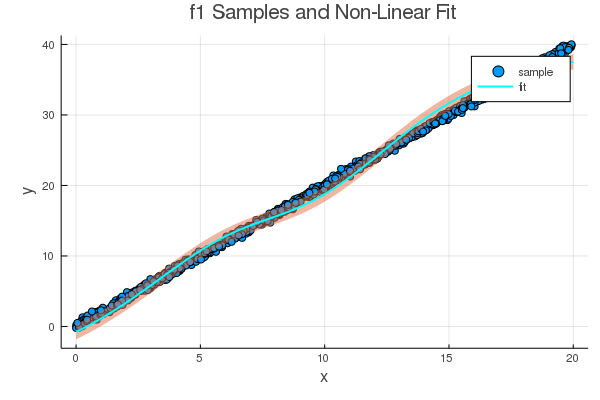
\includegraphics[width=12cm,keepaspectratio]{imgs/2_5_3_4_1.png}
  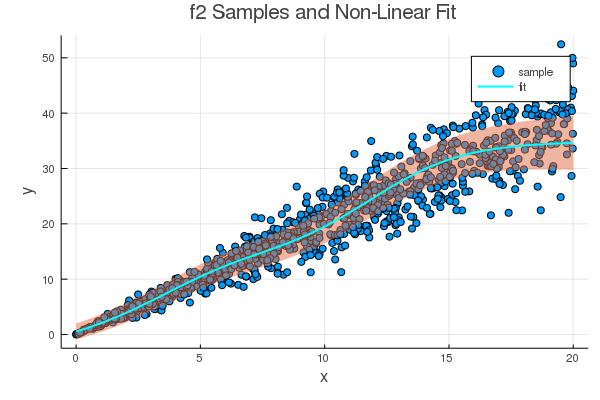
\includegraphics[width=12cm,keepaspectratio]{imgs/2_5_3_4_2.png}
  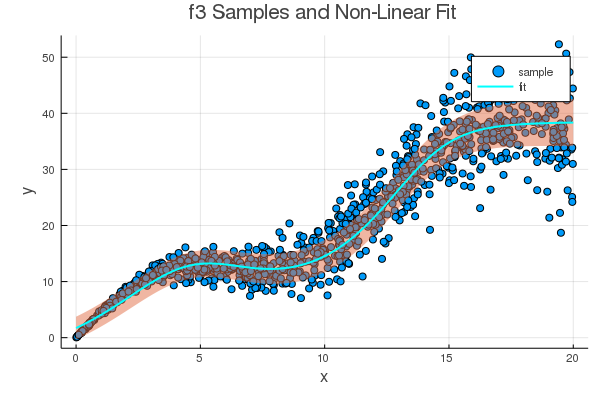
\includegraphics[width=12cm,keepaspectratio]{imgs/2_5_3_4_3.png}
\end{figure}
\end{enumerate}

\end{document}